\chapter{Introduction}
\label{sec:intro}

OpenStack is an opensource project that aims at developing a complete cloud
management system. Similary to the reference architecture described in the
previous Section, it is composed of several services, each one dealing with a
particular aspect a CC infrastructure as depicted in Figure~\ref{fig:openstack}.

\begin{figure}[htbp]
        \centering
        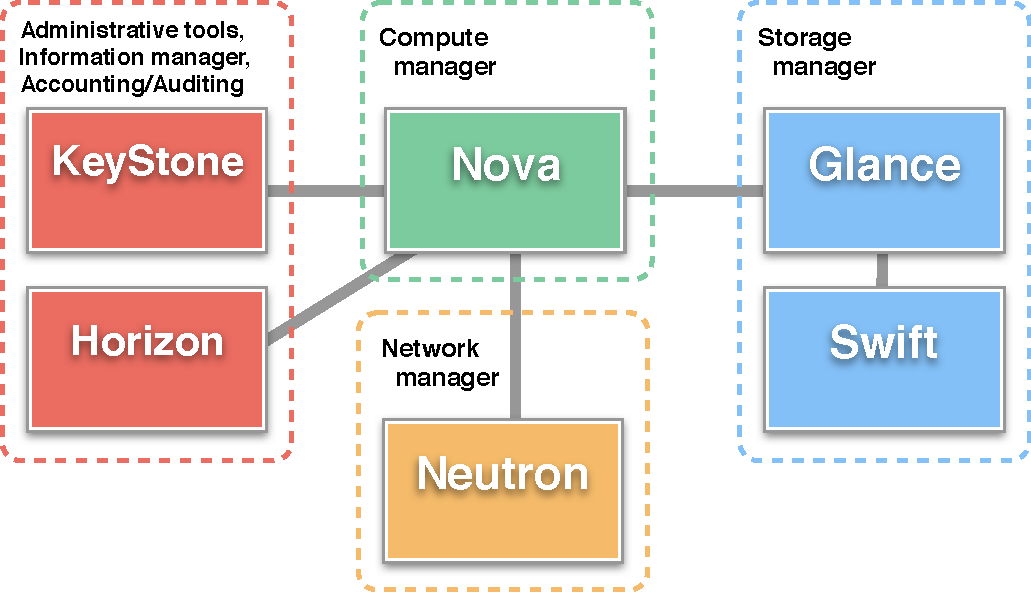
\includegraphics[width=6cm]{figures/OpenStack_architecture.pdf}
        \caption{Services composing OpenStack.}
        \label{fig:openstack}
\vspace*{-.3cm}
\end{figure}


OpenStack relies on two kinds of nodes: controller and compute node. The former
is in charge of managing and distributing work to the latter that provides
computing/storage resources to end-users. In other words, the controllers
correspond to the different services introduced in the previous section while
the compute nodes host the VMs. From the software point of view, the OpenStack
architecture is based on the ``shared nothing" principles: each controller (\ie
each service) is connected to the others via two different way:

\begin{itemize}
   \setlength{\itemsep}{0pt}
  \setlength{\parskip}{0pt}
   \setlength{\parsep}{0pt}
\item \textbf{A messaging queue} that enables the collaboration between sub-services of a
  controller.
\item \textbf{A SQL database} (DB) that stores inner states of a controller.
\end{itemize}

OpenStack's controllers interact with each other through REST APIs or directly
by accessing the inner-state that are stored in the differents DBs. The
architecture used for the Nova service has been organised in a way which ensures
that each of its sub-services does not directly manipulate the database: they
have an indirect access through a service called ``nova-conductor" which in turn
works with an implementation of the \textbf{"nova.db.api"} programming
interface. Developers of Nova provide an implementation of this interface that
is using \textit{SQLAlchemy} to manipulate a relational database. We developed a
second implementation of this interface that replaces every call to the
\textit{SQLAlchemy} by a call to a custom RIAK driver. This enables to make
Nova's services working with RIAK by only changing the database driver: this
limits the level of intrusiveness in the original source code.
